\chapter{Motor Test} \label{chpt:motor_test}
As presented in \cref{sec:laser} the laser unit is composed of an \gls{nxt} and accompanying motors which are part of the Lego Mindstorms series. Two of these motors are needed by the laser unit in order to control the laser both horizontally and vertically. It is assumed that the motors are very imprecise and it is therefore necessary to test and analyse the consistency of the motors. The results of the tests can be used to determine which motors are optimal to use and how to handle or even remove uncertainties.

This chapter presents the attributes that the motors are tested for and how the tests are structured. Error sources that could possibly influence the data are presented, and ways of minimising or removing these error sources is described in the structure of the tests. The data from the tests is also presented and analysed in the chapter.

\section{Goals of Testing}\label{sec:test_goals}
The tests are conducted in order to measure three properties; maximum speed, acceleration and brake speed. Besides testing these three aspects the consistency of them all is also tested. The data acquired from the tests is used to determine which motors that exercise the most consistency. There are four motors to be tested, indexed one to four. The number of the motors stays the same throughout the tests, meaning motor 1 is the same motor for all tests.

As explained in \cref{sc:rig}, a total of two motors are needed in the construction of the rig, where these motors are used for the horizontal and vertical axis'. The motors need to turn a pointer in collaboration, to target an object in a 3D room, which affords the need for moving the motors precisely. If a motor has an imprecision of a few degrees, the effect of this imprecision becomes greater as the distance to the target increases. The existence and size of such imprecision and the consequences hereof must be identified when analysing the data.

In order to fulfil the test goals, a single test is conducted which is a speed-timing test. The speed-timing test measures how long it takes to reach maximum speed and how long it takes to get to a full stop from maximum speed. These measurements can be used to obtain the acceleration, maximum speed and negative acceleration. A last aspect is to analyse the consistency of the runs to get an indication of which motors might be the best to use.

\section{Error Sources}\label{sec:error_sources}
A number of error sources are considered while designing and performing the tests, since there is a risk they can have an effect on the results. Some of these error sources occur as a result of using the selected hardware components, as an example there is a significant backlash in the motors. Another source is the test conductor while a third source is the software used to run the test. The sources are put into three categories; human based, hardware based and test structure based sources. These sources can affect the conclusions of the conducted tests and therefore the associated challenges must be identified.

\subsection{Human Based Sources}
A human based error source is the test conductor. Involving a person in a test may result in human mistakes being made, for example wrongly recording test data or not strictly following the test procedure. By automating tasks, and creating precise descriptions of the test procedures, this uncertainty can be eliminated. But as soon as a person is involved, the uncertainty cannot be entirely eliminated.

\subsection{Hardware Based Sources}
Two hardware based error sources manifest themselves in motor backlash and the internal counter. Because of the quality of the used motors, the precision of their internal components or the size of the backlash cannot be guaranteed.

The first source is the backlash in the motors. It is important that there is a test procedure that either minimises this backlash or makes it a constant value. If this source can be minimized it is more preferred than having a constant factor of backlash in the measurements. Having a constant value for backlash makes it possible to adjust the data if this is known. A problem is that the size of a constant factor can be hard to determine if other error sources are present and therefore the data will be harder to be proper analysed. Therefore it is preferred that the backlash is minimised since the size of the backlash must be obtained.

The second source is internal counter of the motors that counts the number of ticks the motor has moved in a given direction and there might be uncertainties when it reads the tick value. This source is hard to eliminate since it is the equipment used for measuring how much the motor has moved. The size of this reading uncertainty can be estimated if the backlash is eliminated. If backlash is not eliminated the combined effect of the internal counter of the backlash can be measured.

\subsection{Test Structure Based Sources}
There are three error sources that are based on the test structure and test setup. The first is rig structure, which is described in \cref{sc:rig}. The motors are tested while being integrated in this construction.

By including the motors the conditions for the test is the same as when the motor is implemented in a solution. The motors will pull the same weight as if they were included in the final version. This results in data that gives a better foundation for determine which motors are best. A problem is that the construction of the rig can differ between tests of motors. If it does the motors might pull different weights which might affect the data. Two things can be done to minimise this source's impact; having a clear definition of the rigs structure and to have a single test conductor. The last might result in the same structure in all tests but might not be enough to eliminate this source.

A second source is errors in test software. The used software can contain errors resulting in unexpected behaviour. These errors might not be observable while running the test. Therefore the test software should be validated and its behaviour should be tested so it pays respect to its specification, and thereby securing its correctness.

\subsection{Handling Error Sources}
Most of the error sources can either be minimised or eliminated if the test procedure is properly structured, defined and executed. The impact of the sources can be analysed when the results of the tests is obtained. By having identified these error sources it must be part of the data analysis to determine whether or not they had an influence on the data and if so to what extend.

\section{Speed-Timing Test}
In \cref{sec:test_goals} one test was defined as a speed-timing test. This test's purposes are to measure the time used to meet maximum speed, what the maximum speed is and how long time it takes to reach a full stop. This section then presents the test's hypothesis, test structure, data analysis and conclusion.

\subsection{Hypothesis and Test Structure}\label{subsec:acc_test_hyp}
Before presenting the structure of the test structure a hypothesis must be defined. The structure is based in the hypothesis since the data must prove or disprove the hypothesis where the hypothesis is based on the purpose of the test. The hypothesis for this test contains three parts:
\begin{enumerate}[label=\alph*)]
    \item The speed before the motor reached its maximum speed is linear in growth.
    \item When maximum speed is reached the speed will be constant, and not oscillating, until the motor is instructed to brake.
    \item The negative acceleration when braking is linear.
    \item The motor's positive and negative accelerations are the same size.
\end{enumerate}

The three parts are based on assumptions of how the data is formed. In order to prove of disprove the claims the test structure is designed to measure the distance covered at any point in time. From this data the speed can be obtained and from speed the acceleration can be obtained. Having this information the four parts of the hypothesis can be proved or disproved depending on the results.

The hardware used for this test are the \gls{nxt} from the \acrlong{nxt} series, motors from the same series and the rig constructed in \cref{sc:rig}. The \gls{nxt} used the battery pack from the series which delivers 7.4V. The battery pack is connected to charger. The motor to be tested was included in the setup as the motor responsible for the vertical rotation. Doing so the motor have the weight of the other motor. The alternative was that the motor would not have any weight but this might give other results than having the weight on since less momentum is needed.

The software written for this test had the following structure:
\begin{enumerate}
	\item The tick counter is set to zero.
    \item The motor is instructed to run at full speed.
    \item At every millisecond the tick counter is read and the value stored.
    \item At 250 milliseconds the speed is set to zero and the brake is activated.
    \item At every millisecond the tick counter is read and the value stored.
    \item The test stops at 500 milliseconds.
\end{enumerate}
The test software can be seen in \cref{lst_speed_timing} in the appendix.

This procedure was repeated 250 times for each of the four motors that are available. In order to save the data every test was saved in memory on the \gls{nxt}. When the test was finished the data was send to a secondary device for storage. By doing so there was not writing to secondary memory during the tests but in between the tests. Also it reduces the risk that the test conductor makes errors since he only set the tests up and the rest is automated.

The motors are instructed to turn the same way in every test which reduces the influence of backlash. The first test's data might be altered  but the later tests will start from a position where the backlash is minimised. The source that might have the largest impact is the rig construction. If the rig is not properly put together when the motor is changed the data from the different motors might give very different results. This could remove the possibility of getting trustworthy data.

The presented test structure of the speed-timing test is based on four parts of the hypothesis. Error sources are reduced and the data analysis in the section below must determine whether or not the reduction is a success.

\subsection{Data Analysis}\label{ss:data_anal}
The test structure for the speed-timing test gave 250 data sets. This gives 250 data points for each millisecond. In order to work with this the median value for each data point was selected so there instead was one data point for each millisecond. This data set can easily be plotted and a fit can be made.  Then it can be determined if the accelerations is linear in growth. The test software used to record these data points have been reviewed multiple times and been deemed sufficiently correct to guarantee the data to be acceptable for analysing the motors. All figures shown are for motor 1 but all figure for all motors can be seen in \cref{app:res}.

In \cref{fig:data_fit_1} the data for motor 1 is plotted together with a piece wise plot fit. The figure shows the number of degrees the motor has moved at each millisecond, which gives the distance covered at any given time. The data points until maximum speed have a polynomial fit of second order and the same is the data points at negative acceleration. When maximum speed was reached it is linear fit and the same when the brake is finished.

\begin{figure}[!htb]
    \centering
	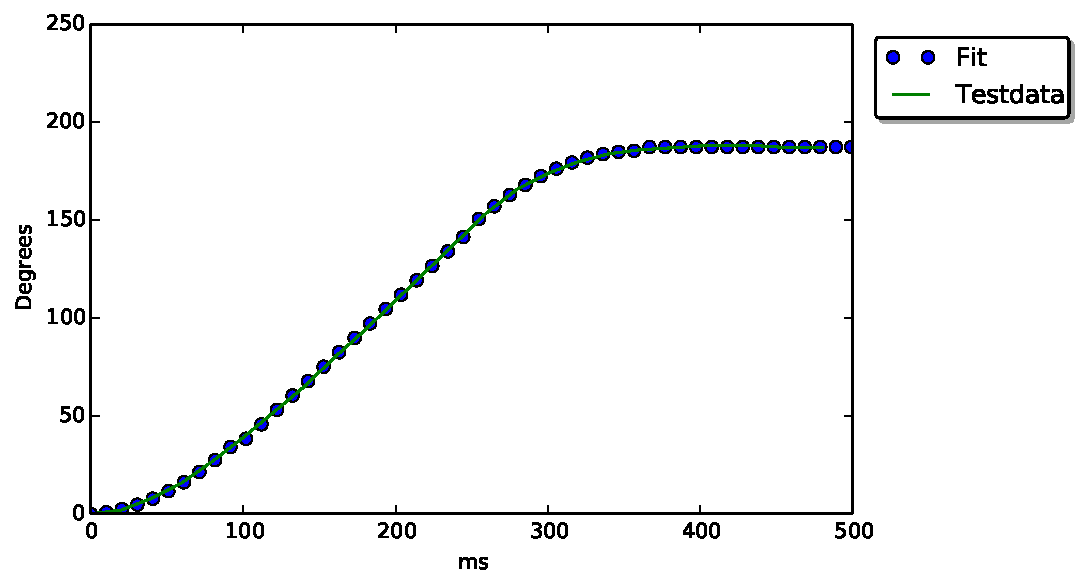
\includegraphics[width=1\textwidth]{test_res/speed_tests/Data_and_fit_motor1.pdf}
     \caption{Test data for motor 1 for the speed-timing test}
	\label{fig:data_fit_1}
\end{figure}

It is no surprise that it is a linear fit when the brake is completed since no more distance is covered. This function for this fit for all for motors is just a constant where the constant is the mean value of the data within the fit's data range. The first increase in instance and when braking are both fitted with a polynomial fit of second order which is consistent with constant acceleration. The distance covered after maximum speed was reached until the brake is introduced the fit is also linear. All of fits made for all the four motors have an R\textsuperscript{2}-value that is above 0.99. Having such a high value means that a fit of higher order is not needed. Now having these piece wise plot fit consisting of four parts it is possible to analyse the speed speed at any given moment. The plot fit was differentiated and is shown in \cref{fig:speed_1}.

\begin{figure}[!htb]
    \centering
	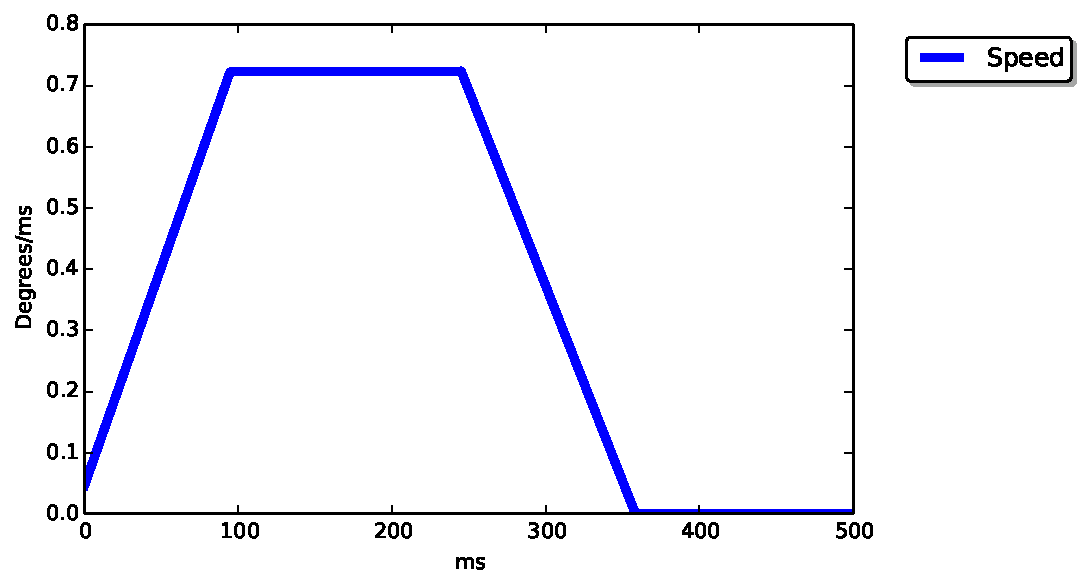
\includegraphics[width=1\textwidth]{test_res/speed_tests/Speed_motor1.pdf}
     \caption{Speed at any given time for motor 1 for the speed-timing test}
	\label{fig:speed_1}
\end{figure}

One thing to notice is how the first plot fit crosses the y-axis and does not cross point $(0,0)$. This is due to fit not being a perfect fit but since the R\textsuperscript{2}-value is above 0.99 this is accepted. The plot might have a better fit if the order was higher and therefore start in point $(0,0)$. A problem that could arise by having a higher order is when the fit is differentiated to get the speed and the acceleration. By having a higher order the speed and acceleration could appear to oscillate in the tests. This fluctuation might be unobservable if a very high order is used and it would give a more smooth transition between the four functions used to fit the data in \cref{fig:speed_1}. Otherwise the second order fits have a good fit on the data so it is determined that a second order fit is sufficient for analysing the data.

\begin{table}
  \centering
  \begin{tabular}{| c | c | c |}
    \hline
    Motor Id & Max speed reached at & Max speed in Degrees/ms   \\ \hline
    1 & 95 ms & 0.723 \\ \hline
    2 & 95 ms & 0.723  \\ \hline
    3 & 100 ms & 0.730 \\ \hline
    4 & 94 ms & 0.716   \\ \hline
  \end{tabular}
  \caption{The maximum speed for the speed timing test}
  \label{tbl:max-speed}
\end{table}

From \cref{fig:speed_1} and the plot fits for the three other motors the maximum speed is obtained. In \cref{tbl:max-speed} the time taken to reach maximum speed is listed including the speed itself. Motor 3 is the only motor that notably differs from the other motors in the time it takes to reach maximum speed. Otherwise it is noted that the might be a relation between the size of the speed and the time it takes to reach it. The less time used to reach the speed the less the speed is. This speed does not make it clear which motors to use. The distance the motors cover in 10ms at maximum speed is 7.x degrees. The resolution for internal counter is 1 degree so the difference would be unobservable. If the motor are on for a longer time the difference would be observable but acceleration and consistency of the motors must be determined before the maximum speed can be used.

\begin{figure}[!htb]
    \centering
	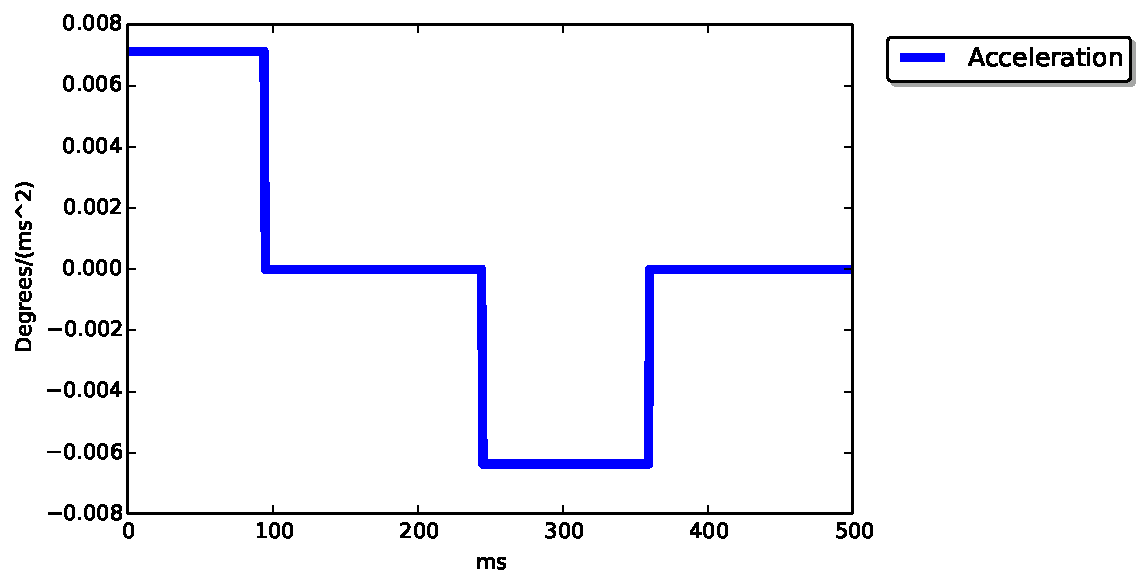
\includegraphics[width=1\textwidth]{test_res/speed_tests/Acc_motor1.pdf}
     \caption{Acceleration at any given time for motor 1 for the speed-timing test.}
	\label{fig:acc_1}
\end{figure}

The acceleration for motor 1 is shown in \cref{fig:acc_1}. The acceleration is constant for all four piecewise plots. The acceleration when maximum speed and full stop is reached is 0 since the speed in constant. In \cref{tbl:acc} all the positive and negative accelerations are presented. Every motor's positive acceleration is greater than its negative acceleration. The ration between the motors' two accelerations are between 0.90 to 0.94. Therefore it can not be said that in the general case that the accelerations are of the same size.

\begin{table}
  \centering
  \begin{tabular}{| c | c | c |}
    \hline
    Motor Id & Positive acceleration in degrees/ms\textsuperscript{2}& Negative acceleration in degrees/ms\textsuperscript{2}  \\ \hline
    1 & 0.00712 & -0.00637 \\ \hline
    2 & 0.00701 & -0.00662  \\ \hline
    3 & 0.00677 & -0.00630 \\ \hline
    4 & 0.00703 & -0.00636   \\ \hline
  \end{tabular}
  \caption{The positive and negative accelerations for the speed timing test}
  \label{tbl:acc}
\end{table}

Before concluding on any of the data the standard deviation is considered. In \cref{fig:standard_1} the standard deviation for motor 1 is shown. For the most part the deviation follows a linear growth up until the 300 milliseconds mark which suggest a constant value being applied every millisecond. For all four motors there is a high increase in deviation for the first 10 milliseconds where there rise becomes linear. When the motors is instructed to brake the size of the increase falls and there is no longer any increase when the motors has reached full stop. This means that increase in deviation is linear in time at maximum speed and while the motors has a positive acceleration.

Backlash does not explain why the deviation increases over time. It would explain a deviation the first data point was read but after that the motor would have moved past the backlash. An increasing in deviation could indicate that the constant values for speed and acceleration changes throughout the test runs. If two tests have different values the difference in distance covered would increase as more time parses. As the difference increases over time the standard deviation would do the same. If the values are different between test runs the voltage delivered to the motor has changed between tests. The tests was done with a battery pack connected to the charger. Since the battery pack is a lithium battery the voltage decreases over time. Running tests lower the battery charge but the battery would when be charged, which could result in an oscillating size of voltage. A change in 0.005 degrees/ms\textsuperscript{2} gives a difference of 1 degree after 200 milliseconds which would require an increase of 5-6\textperthousand\ is needed. Since only a small change in voltage is needed to create the observed deviation an oscillating voltage could be the error source.

Another source explaining the increases of standard deviation over time could be the internal tick counter in the motors. If the counter has a constant risk of missing a tick it would result in a linear growing standard deviation. This error source is far less preferable than having a battery pack that changes it voltages. If ticks are missed by the counter it is not possible for the counter to observe the miss and thereby recover from it and the motors might be calibrated more often. If the source for changes in deviation is the battery pack the power source can be changed to a constant voltage which would remove the linear growth in deviation.

\begin{figure}[!htb]
    \centering
	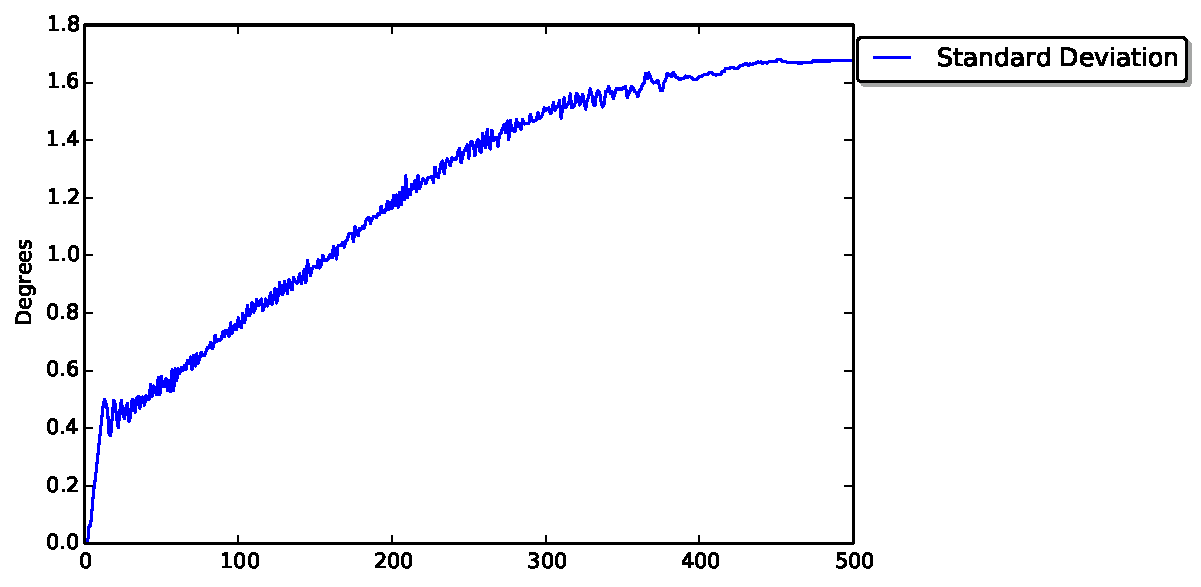
\includegraphics[width=1\textwidth]{test_res/speed_tests/StandardDeviation_motor_1.pdf}
     \caption{Standard deviation at any given time for motor 1 for the speed-timing test}
	\label{fig:standard_1}
\end{figure}

\subsection{Conclusion of Speed-Timing Test}\label{subsec:con_speed}
After reviewing the data, it can be seen that all but one of the presented hypothesis holds. The speed before the motor reached its maximum speed was measured to be of linear growth. When maximum speed is reached the speed is constant until the motor is instructed to brake and since the plot fit had a R\textsuperscript{2} of 0.99 the speed is considered to not oscillate. The negative acceleration when braking was measured to be of linear decline. The motors' positive and negative accelerations ratio is too different as the ratio between the accelerations are 0.90 to 0.94.

There is no clear indication of which motors are better than the others from this test. Their values for acceleration and top speed are close to each other. One aspect to where their differ is in standard deviation. If the increase in standard deviation is caused by skipping ticks no amount of calibrating will be successful as the model rapidly deviates from reality. This deviation results in frequent need of calibration if the internal tick counter is used. Rather using the tick counter external means could be used to measure the distance the motor covered.

If the error source is not the tick counter but rather changes in voltage a \gls{pid} as presented in \cref{ss:pid} would compensates for the deviation. This compensation occurs since the \gls{pid} continually approaches a target value. It is estimated that changes in voltage has a higher probability to be the source of errors than the tick counter. If this assumptions holds there is no need to conduct more tests as the \gls{pid} compensates for the motors' standard deviation. If the standard deviation is removed no motor can be said to be better then the others. But considering the deviation motor 3 has a standard deviation of 2.5 where the others deviation is about 1.7. Therefore motor 3 would be the least preferable to use.